\section{Compiler Status}
\begin{frame}
	\frametitle{Compiler Status}
	%Actors
	 \begin{enumerate}
    \item Item1
    \item Item2
  \end{enumerate}
\end{frame}

\section{Reflection}
\begin{frame}
	\frametitle{Reflection}
	%Bad choices due to inexperience
	%and disagrements of subjective value of the langauge, such as readablity, resulting in half solutions
	%Should instead focus on the target groups preferences as it is their opinions is the ones that ultimately counts
	Reasons for bad decisition:
	\begin{enumerate}
    \item Inexperience with the subject
    \item Disagrements in subjective matters
  \end{enumerate}
\end{frame}

\section{Creative realisation}
\begin{frame}
	\frametitle{A creative realisation}
	%Actors instead of functions, spread the responsiblity, an interesting side-effect
	%This encourages the user to model problem with actors, providing transparency of the actual working of the compiler( but not consise, as expressing as a function)
	Actor as substitudes of functions
	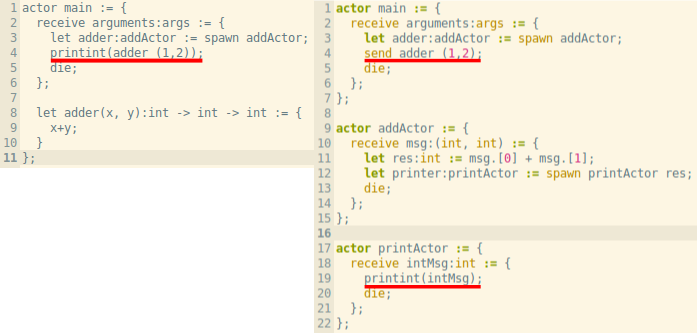
\includegraphics[width=\textwidth]{Images/actorFunc.png}
	But less consise
\end{frame}

\section{Conclusion}
\begin{frame}
	\frametitle{Conclusion}
	%Problemformulering, actors as an solution
	Actors as an solution
	Induces actor modeling as aproaches for modeling the problem
\end{frame}

\section{Future workings}
\begin{frame}
	\frametitle{Future workings}
	Ideas and constructs not included: 
  \begin{enumerate}
    \item Inheritance(OOP)
    \item New construct reply, not having to know the sender locally
    \item Envoriments and iterationSteps
  \end{enumerate}
\end{frame}

\subsection{Environments}
\begin{frame}
	\frametitle{Envoriments}
	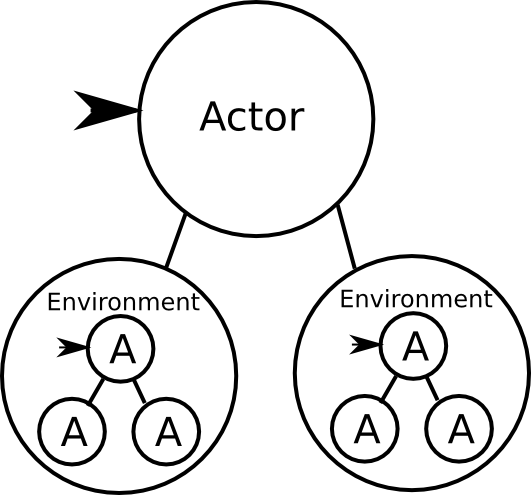
\includegraphics[width=\textwidth/2]{Images/environment.png}
\end{frame}
\subsection{IterationSteps}
\begin{frame}
  \frametitle{IterationSteps}
  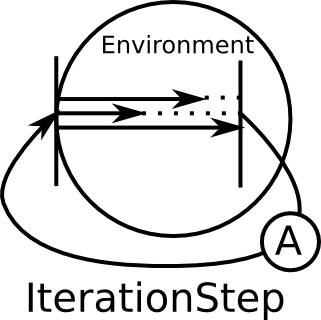
\includegraphics[width=\textwidth/2]{Images/iteration.png}
\end{frame}
